\chapter{Introduction}
\label{sec:intro}
\pagenumbering{arabic}

% Die Einleitung schreibt man zuletzt, wenn die Arbeit im Großen und
% Ganzen schon fertig ist. (Wenn man mit der Einleitung beginnt - ein
% häufiger Fehler - braucht man viel länger und wirft sie später doch
% wieder weg). Sie hat als wesentliche Aufgabe, den Kontext für die
% unterschiedlichen Klassen von Lesern herzustellen. Man muß hier die
% Leser für sich gewinnen. Das Problem, mit dem sich die Arbeit befaßt,
% sollte am Ende wenigsten in Grundzügen klar sein und dem Leser
% interessant erscheinen. Das Kapitel schließt mit einer Übersicht über
% den Rest der Arbeit. Meist braucht man mindestens 4 Seiten dafür, mehr
% als 10 Seiten liest keiner.

\todo{adopt title page}

\todo{adopt disclaimer}

\todo{write introduction}

\section{A Section}

Referencing other chapters: \ref{sec:state} \ref{sec:design}
\ref{sec:implementation} \ref{sec:evaluation} \ref{sec:futurework}
\ref{sec:conclusion}

\begin{table}[htp]
  \centering
  \begin{tabular}{lrr}
    \textbf{Name} & \textbf{Y} & \textbf{Z} \\
    \hline
    \textit{Foo} & 20,614 & \unit[23]{\%} \\
    \textit{Bar} & 9,914 & \unit[11]{\%} \\
    \textit{Foo + Bar} & 30,528 & \unit[34]{\%} \\
    \hline
    \textit{total} & 88,215 & \unit[100]{\%} \\

  \end{tabular}
  \caption[Some interesting numbers]{Various very important looking numbers and sums.}
  \label{tab:numbers}
\end{table}

More text referencing Table~\ref{tab:numbers}.

\section{Another Section}

\begin{figure}[tbp]
  \centering
  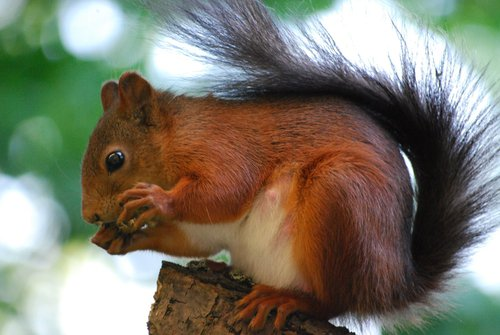
\includegraphics[width=0.8\textwidth]{images/squirrel}
  \caption[Short description]{A long description of this squirrel figure.
  Image taken from
  \url{http://commons.wikimedia.org/wiki/File:Sciurus-vulgaris_hernandeangelis_stockholm_2008-06-04.jpg}}
  \label{fig:squirrel}
\end{figure}

Citing \cite{bellard2005qfa} other documents \cite{bellard2005qfa, boileau06}
and Figure~\ref{fig:squirrel}.

Something with umlauts and a year/month date:
\cite{becher04:_feurig_hacken_mit_firew}.

And some online resources: \cite{green04}, \cite{patent:4819234}

\section{Yet Another Section}

\todo{add content}

\begin{figure}[tbp]
 \missingfigure{Come up with a mindblowing figure.}
 \caption{A mindblowing figure}
 \label{fig:todo}
\end{figure}

\section{Test commands}

\drops \LLinux \NOVA \QEMU
\texttt{memcpy}
A sentence about BASIC. And a correctly formatted one about ECC\@.

\cleardoublepage

%%% Local Variables:
%%% TeX-master: "diplom"
%%% End:
